\section*{Работа с ГИС-картами}
\addcontentsline{toc}{section}{Работа с ГИС-картами}
\subsection*{Доставка с покупками}
\addcontentsline{toc}{subsection}{Доставка с покупками}

\textbf{Задание:}\\
Реализовать модель цепочки поставок ретейлерам, учитывающую то, у ретейлеров имеется покупатели, приобретающие некое количество товаров с использованием ГИС-карт.\\

\textbf{Решение:}\\
Для начала необходимо разместить ГИС-карту и выделить регион -- Франция, так как местоположения ретейлеров и дистрибьюторов находятся именно в этом регионе. (Рисунок \ref{fig:france1})
\begin{figure}[h]
	\centering 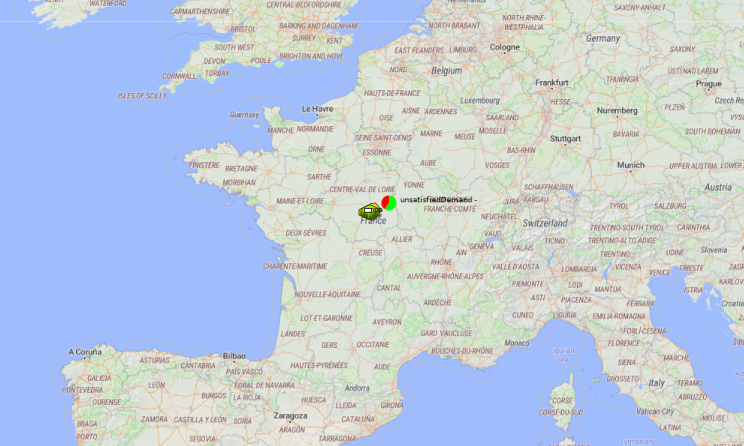
\includegraphics[scale=0.35]{france1}
	\caption{Разметка ГИС-карты}
	\label{fig:france1}
\end{figure}

Также имеются данные о расположении дистрибьютеров и количестве грузовиков, имеющихся в наличии у каждого из дистрибьютеров и данные о местоположений ретейлеров находятся в таблицах, которые импортируются и используются в дальнейшем.\\

Далее создаются несколько популяций агентов: ретейлеров, дистрибьютеров, грузовиков и заказов. (Рисунок \ref{fig:france2})
\begin{figure}[h]
	\centering 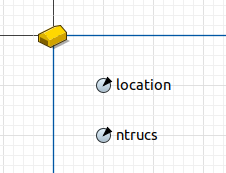
\includegraphics[scale=0.4]{france2}
	\caption{Популяция дистрибьютеров}
	\label{fig:france2}
\end{figure}

\newpage

У дистрибьютеров имеется два параметра: позиция и количество грузовиков, которые у них имеются.\\

У агентов типа <<заказ>> имеется также два параметра: количество товара заказа и ретейлер, который оформил данный заказ. (Рисунок \ref{fig:france3})
\begin{figure}[h]
	\centering 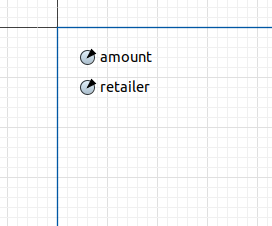
\includegraphics[scale=0.6]{france3}
	\caption{Популяция заказов}
	\label{fig:france3}
\end{figure}

Грузовики имеют несколько состояний: находятся у дистрибьютера, двигаются к ретейлеру, разгружаются у ретейлера, двигаются к дистрибьютеру. (Рисунок \ref{fig:france4})
\begin{figure}[h]
	\centering 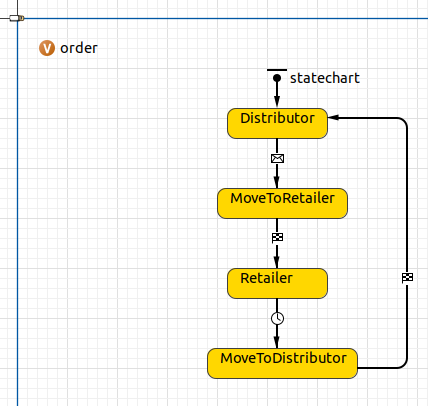
\includegraphics[scale=0.6]{france4}
	\caption{Популяция грузовиков}
	\label{fig:france4}
\end{figure}

\newpage

Грузовик начинает свое движение при получении сообщения. Отправка данного сообщения осуществляется ретейлером, когда достигнут критический запас при помощи событий. (Рисунок \ref{fig:france5})
\begin{figure}[h]
	\centering 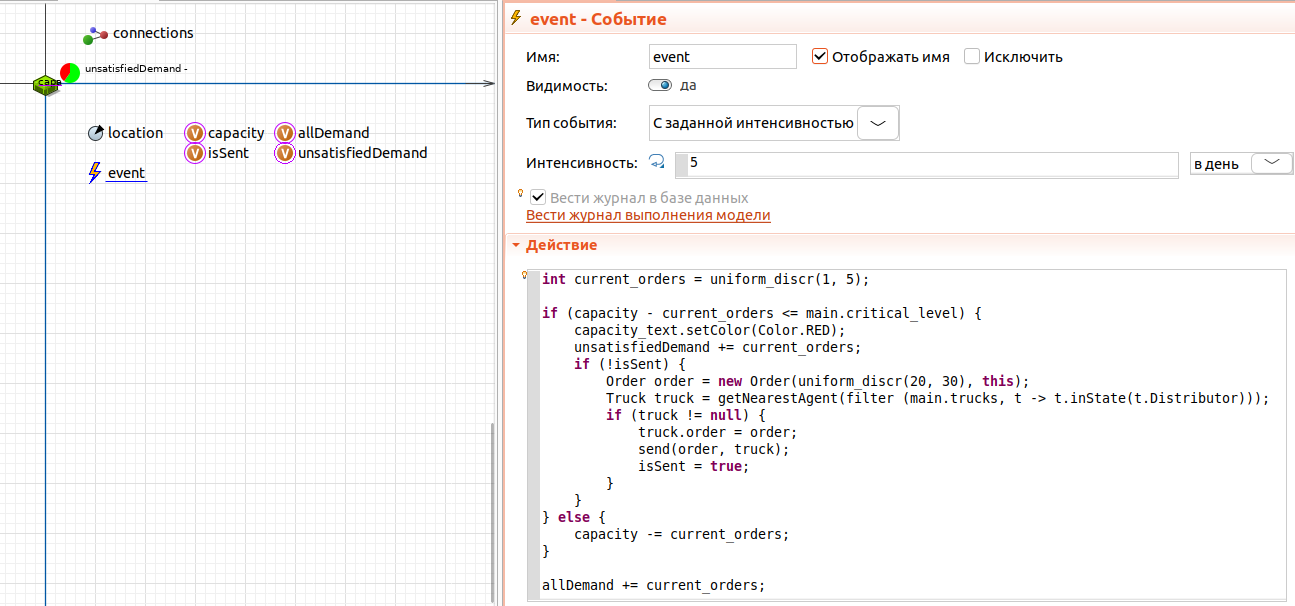
\includegraphics[scale=0.4]{france5}
	\caption{Популяция заказов и логика основного события}
	\label{fig:france5}
\end{figure}

Также у ретейлеров имеется круговая диаграмма, которая отражает количество удовлетворённого и неудовлетворённого спроса, а также имеется метка, которая отражает актуальное число запасов данного ретейлера. (Рисунок \ref{fig:france6})
\begin{figure}[h]
	\centering 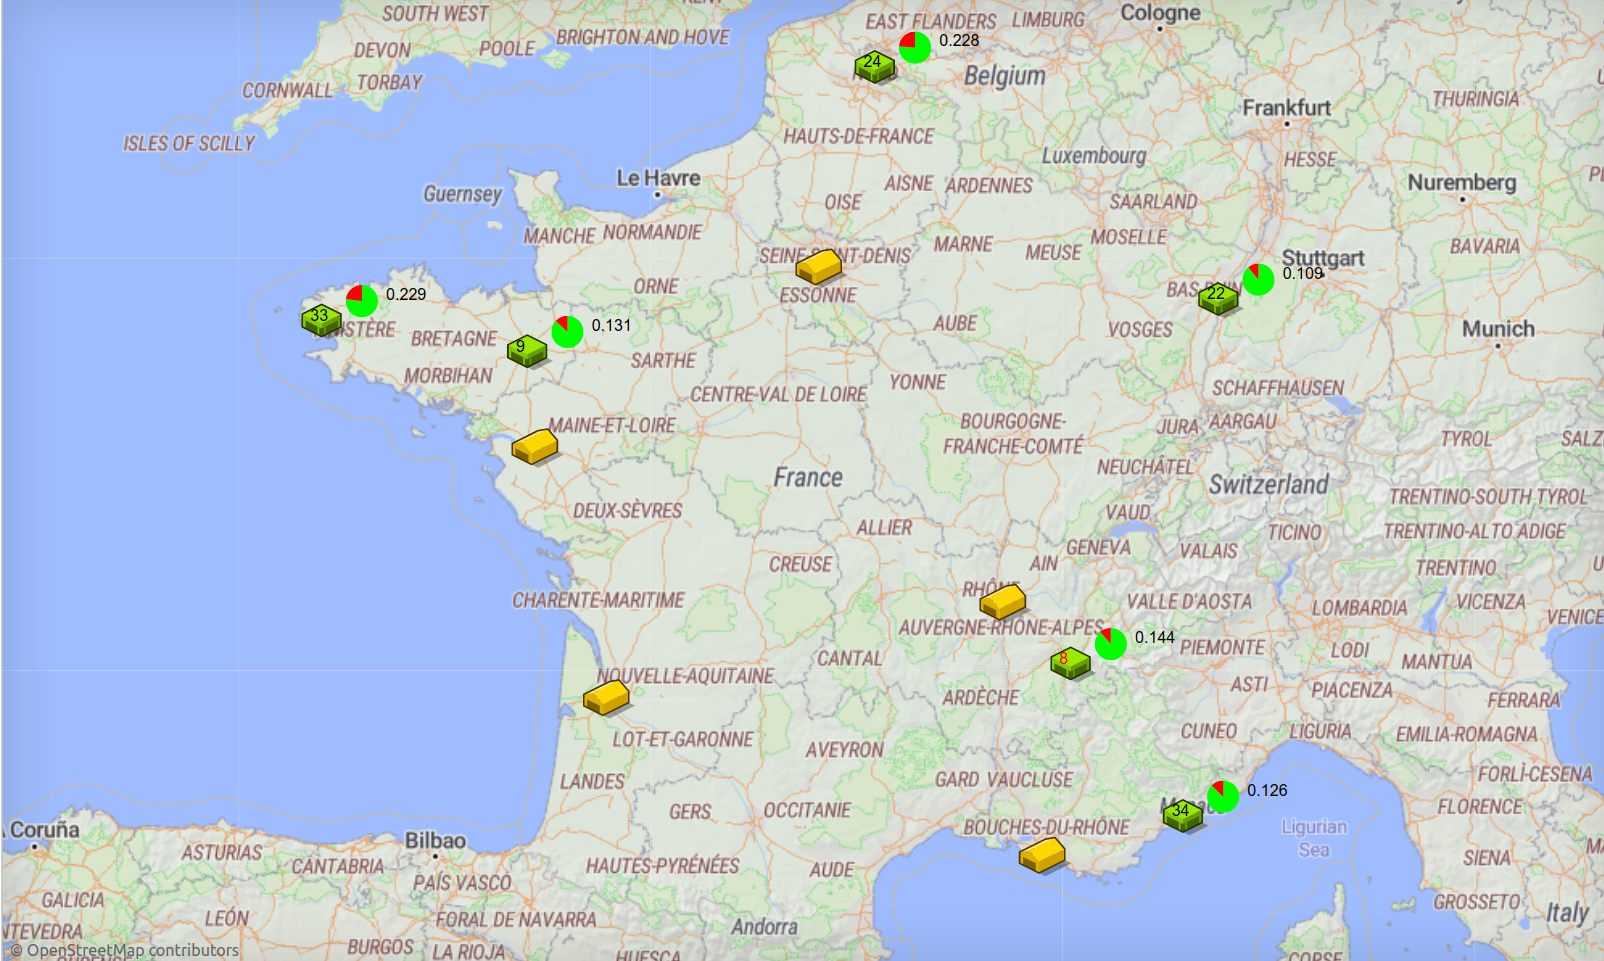
\includegraphics[scale=0.2]{france6}
	\caption{Запуск симуляции модели}
	\label{fig:france6}
\end{figure}

Таким образом, была реализована модель доставки с покупками, на примере которой мы ознакомились с основными механиками работы с ГИС-картами.